\documentclass[20pt,a4paper]{article}

% Language setting
\usepackage[english, french]{babel}

% % Set page size and margins
% % Replace `letterpaper' with `a4paper' for UK/EU standard size
\usepackage[top=2cm,bottom=2cm,left=2cm,right=2cm,marginparwidth=1.75cm]{geometry}

% Useful packages
\usepackage{amsmath}\usepackage{graphicx}
\usepackage{subfigure}
\usepackage{latexsym}
\usepackage{array}
\usepackage[bookmarks, colorlinks=true, pdfborder={0 0 0}, pdftitle={MLRF rapport}, pdfauthor={Elouan Vincent, Quentin Fournel}]{hyperref}
\linespread{1}
\usepackage{titlesec}
\titlespacing{\section}{0pt}{\baselineskip}{0pt} 
\usepackage{fancyhdr}
\usepackage{nccrules}
\usepackage{titlesec}
\usepackage{verbatim}
\usepackage{multirow}
\usepackage{longtable}
\usepackage{float}
\usepackage{enumitem}
\usepackage{pifont}
\usepackage[table]{xcolor}
\usepackage{algorithm} % To include algorithm in your report
\usepackage{algpseudocode}
\usepackage{booktabs}

%%% The flowing line are use for a package that allow to include colored code in the report
\usepackage{listings}
\usepackage{xcolor}
\definecolor{codegreen}{rgb}{0,0.6,0}
\definecolor{codegray}{rgb}{0.5,0.5,0.5}
\definecolor{codepurple}{rgb}{0.58,0,0.82}
\definecolor{backcolour}{rgb}{0.95,0.95,0.92}

\lstdefinestyle{mystyle}{
    backgroundcolor=\color{backcolour},   
    commentstyle=\color{codegreen},
    keywordstyle=\color{magenta},
    numberstyle=\tiny\color{codegray},
    stringstyle=\color{codepurple},
    basicstyle=\ttfamily\footnotesize,
    breakatwhitespace=false,         
    breaklines=true,                 
    captionpos=b,                    
    keepspaces=true,                 
    numbers=left,                    
    numbersep=5pt,                  
    showspaces=false,                
    showstringspaces=false,
    showtabs=false,                  
    tabsize=2
}
\lstset{style=mystyle}
\usepackage{minted} % Another package to include code

\begin{document}
\selectlanguage{english}
\thispagestyle{empty}
 \begin{titlepage}
\fancypagestyle{emptyt}{%
  \fancyhf{}
  \vspace{1cm}
  \fancyhead[L]{Elouan Vincent \& Quentin Fournel - SCIAG 2024}
  \fancyhead[R]{MLRF}
}
\begin{center}
\thispagestyle{emptyt}
\vspace{2cm}

\includegraphics[scale=0.3]{./logo/epita.png}

\vspace{2cm}

\textbf{\Large Projet final - MLRF}
\\[0.2cm]

\vspace{0.4cm}
%\HRule\\[0.3cm]
\hspace{0.3cm}

\begin{center}
\line(2,0){350}\\
\vspace*{0.5cm} \textbf{{\LARGE{CIFAR-10 classification}}}\\
\vspace*{0.5cm}\line(2,0){350}\\
\end{center}

%\HRule \\[0.7cm]
\hspace{0.7cm}

 \large \emph{Auteurs:}\\
\textbf{\Large{Elouan Vincent \\ Quentin Fournel}} \\[1.cm]



\includegraphics[scale=0.22]{./logo/sciag.jpeg}~\\


\vfill
% Bottom of the page

{\large \today}


\end{center}
\end{titlepage}

\newpage
{\linespread{.8}\hypersetup{linkcolor=black}\tableofcontents}
\newpage
\pagenumbering{arabic}
\titlespacing{\chapter}{0cm}{1cm}{2cm}


\fancyhf{}
\fancyhead[RE,RO]{\bfseries\leftmark}
\fancyfoot[LE,LO]{\textit {\raisebox{-7pt}{
\includegraphics[scale=0.02]{logo/sciag.jpeg}} Rapport projet final - MLRF - Elouan Vincent \& Quentin Fournel} } \fancyfoot[RE,RO]{\bfseries\thepage}

\fancypagestyle{plain}{%pages de tetes de chapitre
\fancyhead{}%supprime lentete
\renewcommand{\headrulewidth}{0pt} %et le filet
} \pagestyle{fancy}



\section{Introduction}\label{sec:intro}

Ce rapport présente notre projet de classification d'images sur le jeu de données CIFAR-10. Dans ce projet, nous avons exploré différentes méthodes d'extraction de descripteurs et utilisé des modèles de classification pour prédire les classes correspondantes aux images.

Dans ce rapport, nous présenterons les différentes méthodes d'extraction de descripteurs que nous avons utilisées, à savoir l'image aplatie, l'histogramme de couleur et la méthode "Bag of Visual Words" (BoVW). Nous expliquerons également les modèles de classification que nous avons mis en œuvre, notamment la régression logistique et les K plus proches voisins (KNN).

Nous espérons que ce rapport fournira une compréhension approfondie de notre approche de classification d'images sur CIFAR-10 et présentera les résultats obtenus pour chaque méthode d'extraction de descripteurs et chaque modèle de classification.
\section{Dataset}

Dans le cadre de notre projet, nous avons utilisé le jeu de données CIFAR-10 pour entraîner et évaluer notre modèle. CIFAR-10 est un ensemble de données largement utilisé dans la communauté de l'apprentissage automatique pour la classification d'images.

Le jeu de données CIFAR-10 se compose d'un total de 60 000 images réparties en 10 classes distinctes. Chaque image a une taille de 32x32 pixels et est représentée en couleurs RGB, ce qui signifie qu'elle est composée de trois canaux : rouge, vert et bleu. Chaque canal contient des valeurs de pixel dans l'intervalle de 0 à 255.

Les 10 classes présentes dans CIFAR-10 sont les suivantes : avion, automobile, oiseau, chat, cerf, chien, grenouille, cheval, bateau et camion. Chaque classe compte 6 000 images, réparties également dans l'ensemble d'entraînement et l'ensemble de test.

CIFAR-10 est très populaire et couramment utilisé pour différentes raisons. Tout d'abord, il s'agit d'un ensemble de données bien établi et largement utilisé dans la communauté. De nombreux travaux de recherche et modèles de référence sont basés sur ce jeu de données, ce qui nous a permis de comparer nos résultats à ceux obtenus dans d'autres études.

De plus, CIFAR-10 offre une diversité d'images représentant différentes classes d'objets. Cela nous a permis de tester la capacité de notre modèle à reconnaître et classifier correctement différents types d'objets dans des images réelles.

Enfin, la taille des images dans CIFAR-10 (32x32 pixels) nous a permis de réduire la complexité de nos modèles et de diminuer les besoins en puissance de calcul. Cela nous a offert la possibilité d'itérer rapidement sur différentes paramètres d'apprentissage, ce qui était essentiel pour notre projet.
\section{Méthode}

\subsection{Extraction de descripteur}

\subsubsection{Image applatie}

Dans notre projet, l'une des méthodes d'extraction que nous avons utilisé est la méthode de l'image aplatie afin de traiter les images du jeu de données CIFAR-10 avant de les introduire dans notre modèle de classification.

La méthode de l'image aplatie consiste à convertir chaque image 2D en un vecteur 1D en les dépliant. Normalement, une image couleur dans CIFAR-10 est représentée sous la forme d'un tenseur de dimensions (largeur, hauteur, canaux) où les canaux correspondent aux composantes rouge, verte et bleue (RGB). Cependant, pour pouvoir les utiliser comme entrée dans notre modèle, nous avons transformé ces images en un vecteur unidimensionnel de taille fixe.

Pour applatir les images, nous avons réalisé les étapes suivantes :

\begin{enumerate}
    \item Prétraitement de l'image
    
    \item Aplatissement de l'image : Nous avons réorganiser les pixels de l'image prétraitée en un vecteur unidimensionnel.

    \item Normalisation : Les valeurs des pixels dans le vecteur aplati ont été normalisées en les divisant par 255. Cette étape permet de ramener les valeurs des pixels dans l'intervalle [0, 1], ce qui facilite l'apprentissage du modèle.
    
    \item Transformation non linéaire : Pour améliorer les performances du modèle, nous avons appliqué une transformation non linéaire aux valeurs des pixels en utilisant np.sqrt(). Cette opération permet d'accentuer les différences entre les pixels et de mieux capturer les caractéristiques discriminantes de l'image.
\end{enumerate}

Une fois l'image aplatie, nous l'avons utilisée comme entrée pour notre modèle de classification. Cette méthode d'aplatissement d'image nous a permis de simplifier le traitement des données et de les rendre compatibles avec les couches d'entrée de notre modèle.

L'avantage de cette méthode est qu'elle ne perd pas d'informations significatives sur les images, car elle conserve l'ensemble des pixels et leurs canaux RGB. De plus, l'image aplatie réduit considérablement la complexité des données tout en maintenant leur représentation sémantique.

En utilisant la méthode de l'image aplatie, nous avons pu entraîner notre modèle de classification avec des données d'entrée appropriées et obtenir des résultats satisfaisants dans la tâche de classification d'images du jeu de données CIFAR-10.

\subsubsection{Histogramme de couleur}

Une autre méthode que nous avons utilisée dans notre projet est l'histogramme de couleur. Cette méthode consiste à extraire les informations de couleur d'une image et à représenter ces informations sous forme d'histogramme. L'histogramme de couleur nous permet de quantifier la répartition des couleurs dans une image, ce qui peut être utile pour la classification et la reconnaissance d'objets.

Pour mettre en œuvre cette méthode dans notre projet, nous avons suivi les étapes suivantes :

\begin{enumerate}
    \item Prétraitement de l'image
    
    \item Conversion en niveaux de gris
    
    \item Calcul de l'histogramme de couleur : Nous avons compté le nombre d'occurrences de chaque intensité de pixel dans l'image pour construire l'histogramme de couleur.
    
    \item Normalisation : Pour rendre l'histogramme de couleur indépendant de la taille de l'image, nous l'avons normalisé en le divisant par sa norme euclidienne.
    
    \item Transformation non linéaire : Pour améliorer les performances du modèle, nous avons appliqué une transformation non linéaire aux valeurs de l'histogramme en utilisant np.sqrt(hist).
\end{enumerate}

Pour appliquer cette méthode à l'ensemble des données CIFAR-10, nous avons utilisé la classe ColorHist. Nous avons parcouru les fichiers du répertoire d'entraînement et du répertoire de test, et pour chaque fichier, nous avons calculé l'histogramme de couleur en utilisant les étapes mentionnées ci-dessus. Les histogrammes de couleur et les étiquettes correspondantes ont été stockés dans des listes. Enfin, nous avons converti ces listes en tableaux NumPy pour une manipulation plus efficace.

\subsubsection{Bag of Visual Words}

Enfin, la dernière méthode d'extraction utilisée est  "Bag of Visual Words" (BoVW). C'est une technique populaire dans le domaine de la vision par ordinateur pour représenter les images en utilisant des descripteurs visuels et des modèles de regroupement (clustering).

La première étape de notre approche BoVW consiste à extraire des descripteurs visuels à l'aide de l'algorithme SIFT (Scale-Invariant Feature Transform). Les descripteurs SIFT sont des vecteurs qui capturent des informations clés sur les points d'intérêt des images, tels que les coins, les bords et les textures.

Nous avons stocké les descripteurs SIFT extraits pour chaque image d'apprentissage dans une liste. De même, les descripteurs SIFT pour les images de test ont été eux aussi stockés dans une liste. Ces descripteurs ont été convertis en tableaux NumPy pour une manipulation plus facile.

Ensuite, nous avons appliqué plusieurs étapes de prétraitement sur les descripteurs SIFT. Tout d'abord, nous avons utilisé une mise à l'échelle (scaling) des données en utilisant un StandardScaler pour normaliser les descripteurs. Ensuite, nous avons appliqué une analyse en composantes principales (PCA) pour réduire la dimensionnalité des descripteurs tout en préservant une grande partie de leur variabilité. Cela nous a permis de réduire la dimension des descripteurs SIFT et de les rendre plus compacts.

Puis, nous avons utilisé l'algorithme de clustering K-means pour regrouper les descripteurs SIFT en un certain nombre de "mots visuels" ou "clusters".

Une fois que nous avons obtenu les clusters avec K-means, nous avons utilisé ces clusters pour représenter chaque image par un histogramme de fréquence des mots visuels. Pour cela, nous avons associé chaque descripteur SIFT à son cluster le plus proche, puis avons compté le nombre de descripteurs associés à chaque cluster pour former l'histogramme. Nous avons ensuite effectué une normalisation et une transformation non linéaire sur l'histogramme pour améliorer les performances du modèle.

En résumé, la méthode BoVW consiste à extraire des descripteurs visuels à l'aide de l'algorithme SIFT, à les prétraiter en utilisant la mise à l'échelle et l'analyse en composantes principales, à regrouper les descripteurs en utilisant K-means pour former des mots visuels, et à représenter chaque image par un histogramme de fréquence des mots visuels. Cette approche nous permet de représenter les images de manière compacte et de les utiliser comme entrée pour des modèles de classification ou de recherche d'images.


\subsection{Modèle de classification}
\subsubsection{Régression Logistic}
La régression logistique est une technique de classification linéaire couramment utilisée pour la classification binaire, mais peut également être étendue à des problèmes de classification multiclasse comme c'est notre cas ici. Dans le contexte de la classification d'images sur le jeu de données CIFAR-10, la régression logistique peut être utilisée pour prédire les classes correspondantes aux images.

La régression logistique repose sur le principe de la régression linéaire, où une combinaison linéaire des caractéristiques est utilisée pour prédire une variable cible. Cependant, dans la régression logistique, la sortie de la combinaison linéaire est passée à travers une fonction appelée fonction sigmoïde (ou logistique) pour obtenir une probabilité. Cette probabilité est ensuite comparée à un seuil (généralement 0,5) pour déterminer la classe prédite.

Plus formellement, la régression logistique modélise la probabilité conditionnelle de chaque classe en utilisant l'équation suivante :
\begin{equation}
P(y = c | x) = softmax(Wx + b)
\end{equation}
où $P(y = c | x)$ est la probabilité conditionnelle que l'image $x$ appartienne à la classe $c$, $W$ est la matrice de poids, $b$ est le vecteur de biais et $softmax$ est une fonction qui normalise les scores pour obtenir des probabilités dans un intervalle de 0 à 1.

Hyperparamètres de la régression logistique :
\begin{itemize}
\item Taux d'apprentissage (learning rate) : Il contrôle l'ampleur des mises à jour de poids à chaque étape de l'entraînement. Un taux d'apprentissage élevé peut entraîner une convergence plus rapide, mais risque de sauter le minimum global. Un taux d'apprentissage trop faible peut rendre l'entraînement très lent.
\item Nombre d'itérations (epochs) : Il indique le nombre de fois que l'algorithme va parcourir tout le jeu de données lors de l'entraînement. Plus le nombre d'itérations est élevé, plus le modèle a de chances de converger vers une solution optimale.
\item Taille du batch (batch size) : Il spécifie le nombre d'échantillons utilisés pour calculer la mise à jour des poids à chaque étape d'entraînement. Un batch size plus grand peut accélérer l'entraînement, mais nécessite plus de mémoire.
\item Régularisation L1 ou L2 : La régularisation est utilisée pour contrôler le sur-apprentissage (overfitting) en ajoutant un terme de pénalité aux poids de la fonction de coût. La régularisation L1 favorise les solutions parcimonieuses en poussant certains poids à zéro, tandis que la régularisation L2 limite la taille des poids.
\end{itemize}

Dans notre cas, nous n'avons pas utilisé de batch, les seuls hyperparamètres sur lesquels nous pouvons jouer pour augmenter les performances d'une régression logistique sont donc le taux d'apprentissage, le nombre d'itérations et la régularisation.

\subsubsection{KNN}

Le KNN est une méthode de classification non-linéaire qui se base sur la similarité entre les échantillons. L'idée principale est de trouver les k échantillons les plus proches (voisins) dans l'espace des caractéristiques pour déterminer la classe d'un nouvel échantillon.

On pourrait définir l'algorithme de la manière suivante :
\begin{enumerate}
\item Calcul de la distance : Dans un premier temps, il faut calculer la distance entre l'échantillon à classer et tous les autres échantillons du jeu de données. On peut utiliser ici la distance que l'on souhaite.
\item Sélection des k plus proches voisins : Les k échantillons ayant les distances les plus faibles sont sélectionnés comme les plus proches voisins.
\item Classification : Parmi les k plus proches voisins, la classe la plus fréquente est déterminée. C'est cette classe majoritaire qui sera attribuée à l'échantillon à classer.
\end{enumerate}

Les KNN n'ont donc pas de réelle phase d'apprentissage, car elle ne possède aucun paramètre, mais dépend des autres données du dataset pour faire sa prédiction.

Cependant, les KNN dépendent de quelques hyperparamètres:
\begin{itemize}
\item Nombre de voisins \textbf{K}: C'est le nombre d'instances les plus proches qui seront prises en compte pour déterminer la classe d'une nouvelle instance. Le choix de cas peut être très important, si sa valeur est trop petite, cela peut entraîner une sensibilité excessive aux \textit{outlayers}, si sa valeur est trop grande, cela risque de trop lisser les frontières de décision et de ne plus donner de résultat pertinent.
\item Métrique de distance : Comme dit précédemment, on peut utiliser plusieurs métriques différentes pour calculer les distances entre les instances. Le choix de la métrique est souvent fait en fonction des données que l'on manipule. La plus utilisée est la distance Euclidienne, mais on peut parfois retrouver la distane de Manhattan ou la distance Minkowski. Dans le cas de classification d'image, ces dernières ne semblent pas pertinentes, nous allons donc nous contenter de la distance Euclidienne.
\item Stratégie de vote : Au moment de déterminer la classe d'une nouvelle instance, un "vote" est fait pour déterminer la classe en fonction des $k$ voisins. Plusieurs stratégies de vote existent. On peut choisir le vote majoritaire, où la classe la plus fréquente l'emporte, ou encore un vote pondéré, où les voisins les plus proches ont plus d'influence.
\end{itemize}

Etant donné la complexité des images CIFAR-10 et la dimension élevée de l'espace des caractéristiques, le KNN peut être moins performant que les autres méthodes. Néanmoins, il peut être utilisé comme une référence de performance ou comme une méthode de base pour comparer avec d'autres algorithmes de classification.

\subsubsection{Random Forest}

Les Random Forest sont une technique d'apprentissage supervisé ensembliste non-linéaire qui combine plusieurs arbres de décision pour effectuer la classification. Chaque arbre de décision est construit sur un échantillon aléatoire du jeu de données d'entraînement, et la classe prédite est déterminée par un vote majoritaire des arbres.
Dans un premier temps, on construit les arbres de décision. Pour chaque arbre, on sélectionne un échantillon tiré au hasard avec remplacement (\textit{bootstrap}) à partir du jeu de données d'entraînement. Ce nouvel échantillon est utilisé pour entraîner l'abre de décision. À chaque nœud de l'arbre, un sous-ensemble aléatoire des caractéristiques est choisi pour diviser les données. Cela permet de réduire la corrélation entre les arbres et d'augmenter la diversité de la forêt.
Une fois tous les arbres de décisions construits, les classes prédites sont déterminées par un vote majoritaire des différents arbres. La prédiction du modèle est la classe qui obtient le plus de vote des arbres de décision.

Un des risques des arbres de décision, et donc des random forest est l'\textit{overfitting}. Il existe plusieurs hyperparamètres dans les random forest donc une bonne partie sert à la régulation du modèle pour éviter l'\textit{overfitting}:
\begin{itemize}
\item Nombre d'arbre: Le nombre d'arbres de décision dans la forêt, un nombre élevé d'arbres dans la forêt peut permettre de meilleur prédiction, mais demande aussi plus de temps de calcul.
\item Profondeur maximale des arbres : C'est la profondeur maximale à laquelle chaque arbre de décision peut se développer. C'est un paramètre de régularisation, car un arbre trop profond peut entraîner un sure apprentissage, mais il ne faut pas que la profondeur maximale soit trop faible au risque d'avoir un modèle sous-performant.
\item Nombre minimum d'échantillon pour diviser un noeuds. Au moment de la construction des arbres de décision, on peut établir un nombre minimal d'instance dans le noeud pour qu'il puisse être divisé. Si un noeud ne compte pas suffisamment d'instance, alors il ne peut pas se séparer et devient une feuille. On retrouve le même paramètre avec un nombre minimum d'instances dans une feuille, évitant d'avoir une feuille ne contenant qu'une instance. Ces deux hyperparamètres sont aussi des hyperparamètres de régularisation.
\end{itemize}

Les random forest sont robustes aux données bruitées, peuvent gérer des ensembles de données de grande dimension et ont une bonne capacité de généralisation. Les Random Forest sont également capables de capturer des interactions non-linéaires entre les caractéristiques. En combinant les prédictions de multiples arbres de décision, elles peuvent fournir des résultats précis et stables. Cependant, il est important de noter que les Random Forest peuvent être plus lentes à entraîner et à prédire que d'autres algorithmes plus simples comme la régression logistic ou les KNN.
\section{Results}
L'implémentation des différentes méthodes présentées dans ce rapport est disponible sur \href{https://github.com/ElouanV/mlrf-sciag-2024}{GitHub}, où vous pourrez retrouver davantage de figures ainsi que reproduire les résultats que l'on vous présente ici. Pour les modèles, nous avons utilisé la librairie \href{https://scikit-learn.org/stable/}{Sklearn}

Nous avons ici comparé les trois modèles en utilisant les trois méthodes d'extraction de features sur chaque modèle. Dans un premier temps, nous comparons les résultats avec les hyperparamètres par défaut de \textit{Sklearn} pour comparer les différentes méthodes.
Ensuite, nous étudierons plus en détails chaque méthode avec les modèles qui a le mieux performé pour affiner les hyperparamètres pour chaque méthode d'extraction de feature.

Les modèles que nous présentons ici ont été entraînés sur l'ensemble des données d'entraînement, c'est-à-dire 50 000 instances et les résultats présentés sont les scores obtenus sur l'ensemble de tests de 10 000 instances. Pour la sélection fine des hyperparamètre, nous avons utilisé la \textit{GridSearch} implémenté dans \textit{Sklearn} avec 3 cross-validation.

Nous évaluerons nos modèles en regardant l'accuracy, la courbe ROC ainsi que la matrice de confusion.

\begin{table}[ht]
\centering
\begin{tabular}{|c|c|c|c|}
\toprule
Model & Flatten & Color Histrogram & BoVW \\
\midrule
LogisticRegression& 34.47\% & 23.01\%&\textbf{20.41\%} \\
KNN & 34.15\%& 22.68\%& 13.34\% \\
RandomForest & \textbf{47.01\%} & \textbf{26.61\%} & 18.26\% \\
\bottomrule
\end{tabular}
\caption{Accuracy de chaque modèle sur chaque méthode d'extraction sans affinage des hyperparamètres sur le jeu de donnée CIFAR-10}
\label{tab:result_no_ft}
\end{table}
Le tableau \ref{tab:result_no_ft} présente l'accuracy de chaque modèle sur chaque méthode d'extraction sans affinage des hyperparamètres. La première chose qui saute aux yeux est le fait que la méthode d'extraction de feature le plus élaboré, \textit{BoVW}, produit les résultats les moins intéressants. On observe un accuracy deux fois plus élevée avec le meilleur utilisant l'image aplatie par rapport au meilleur modèle utilisant \textbf{BoVW}. Sur \textit{BoVW}, la régression logistique semble obtenir les meilleurs résultats.
D'autre part, le KNN semble ne pas bien marcher sur ce problème, comme nous pouvions l'espérer, car il n'est pas adapté à ce genre de tâche.
En revanche, le modèle random forest obtient les meilleurs résultats sur l'image aplatie (26.61\%) et l'histogramme de couleur (47.01\%).
La figure \ref{fig:confusion} montre les matrices de confusion des meilleurs modèles. La matrice de confusion du random forest sur image aplatie est évidemment plus propre, mais on remarque aussi que la random forest sur l'histogramme de couleur arrive à bien classifier les avions et bateau, et lorsqu'il y a une erreur, ils sont confondu l'un et l'autre. Cela vient probablement du fait qu'ils partagent des caractéristiques communes: souvent l'objet en blanc sur un fond bleu, qui est singulier par rapport aux images de chat, de chien etc. où l'on retrouve un fond vert avec un objet marron.
\begin{figure}
\centering
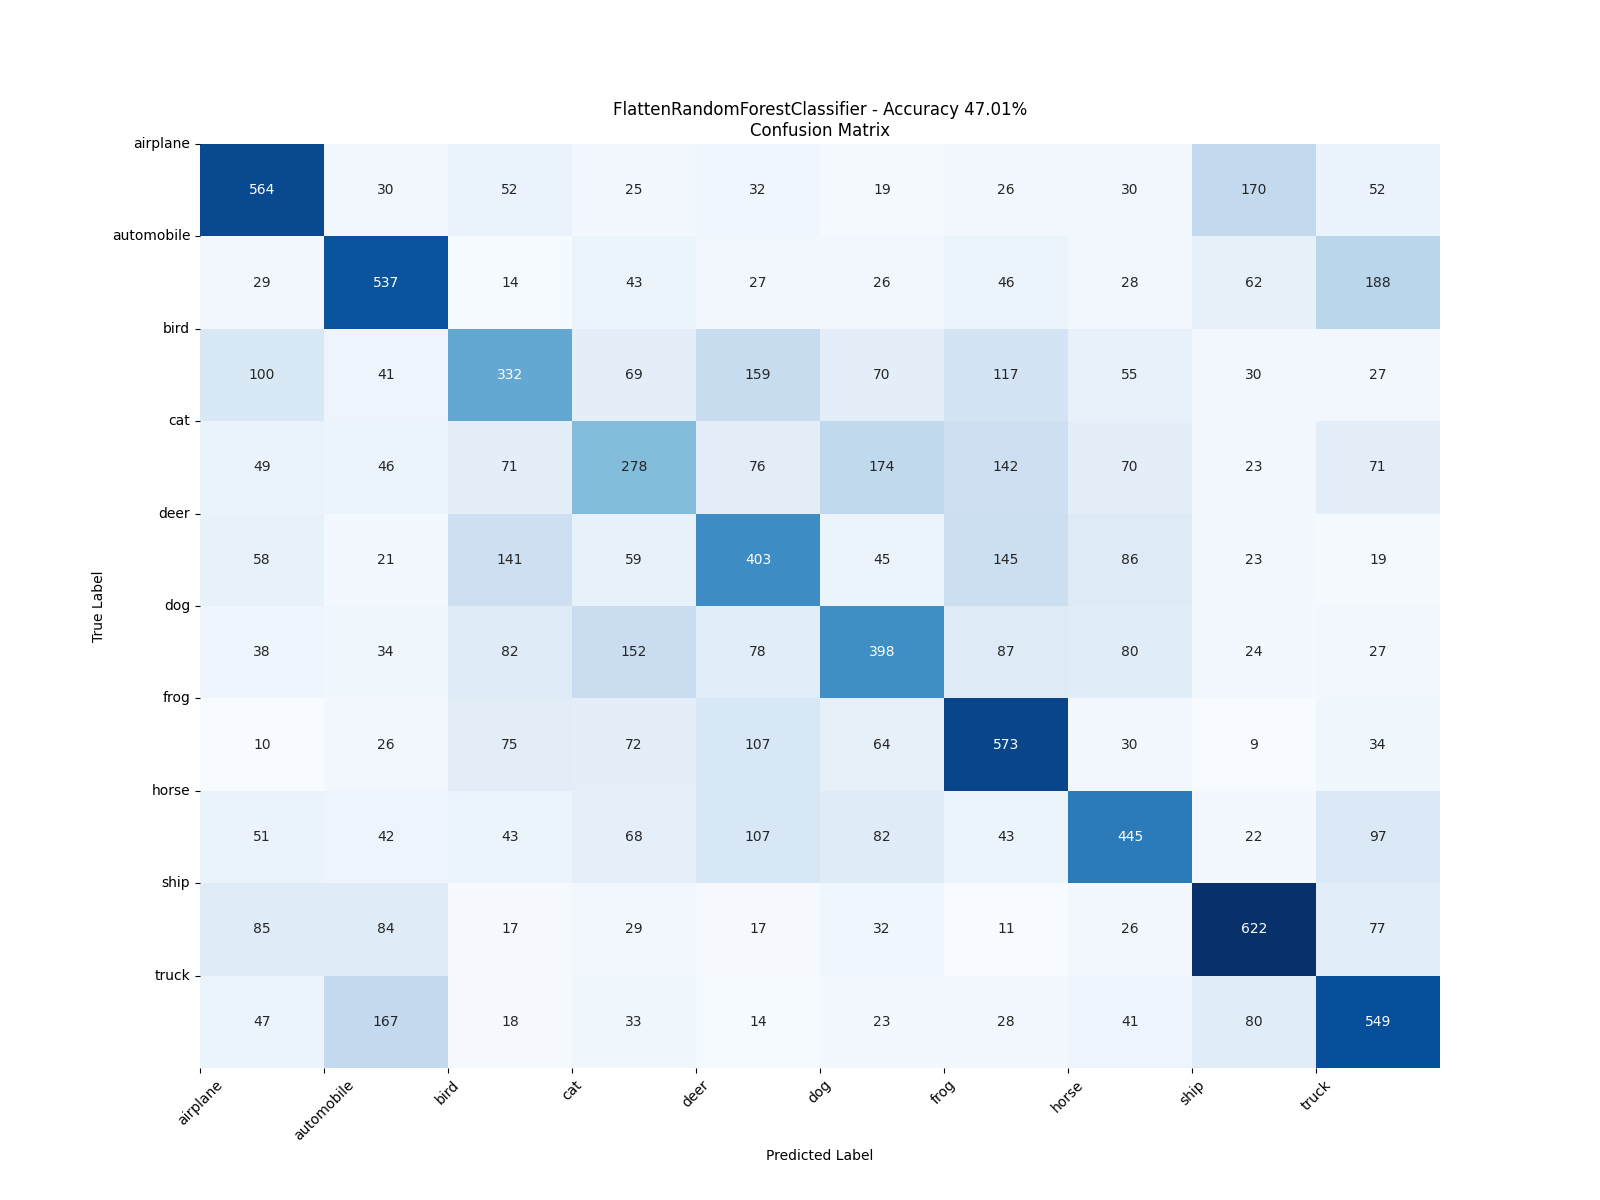
\includegraphics[scale=0.2]{figures/confusion_matrix_RandomForestClassifier_flatten.png}
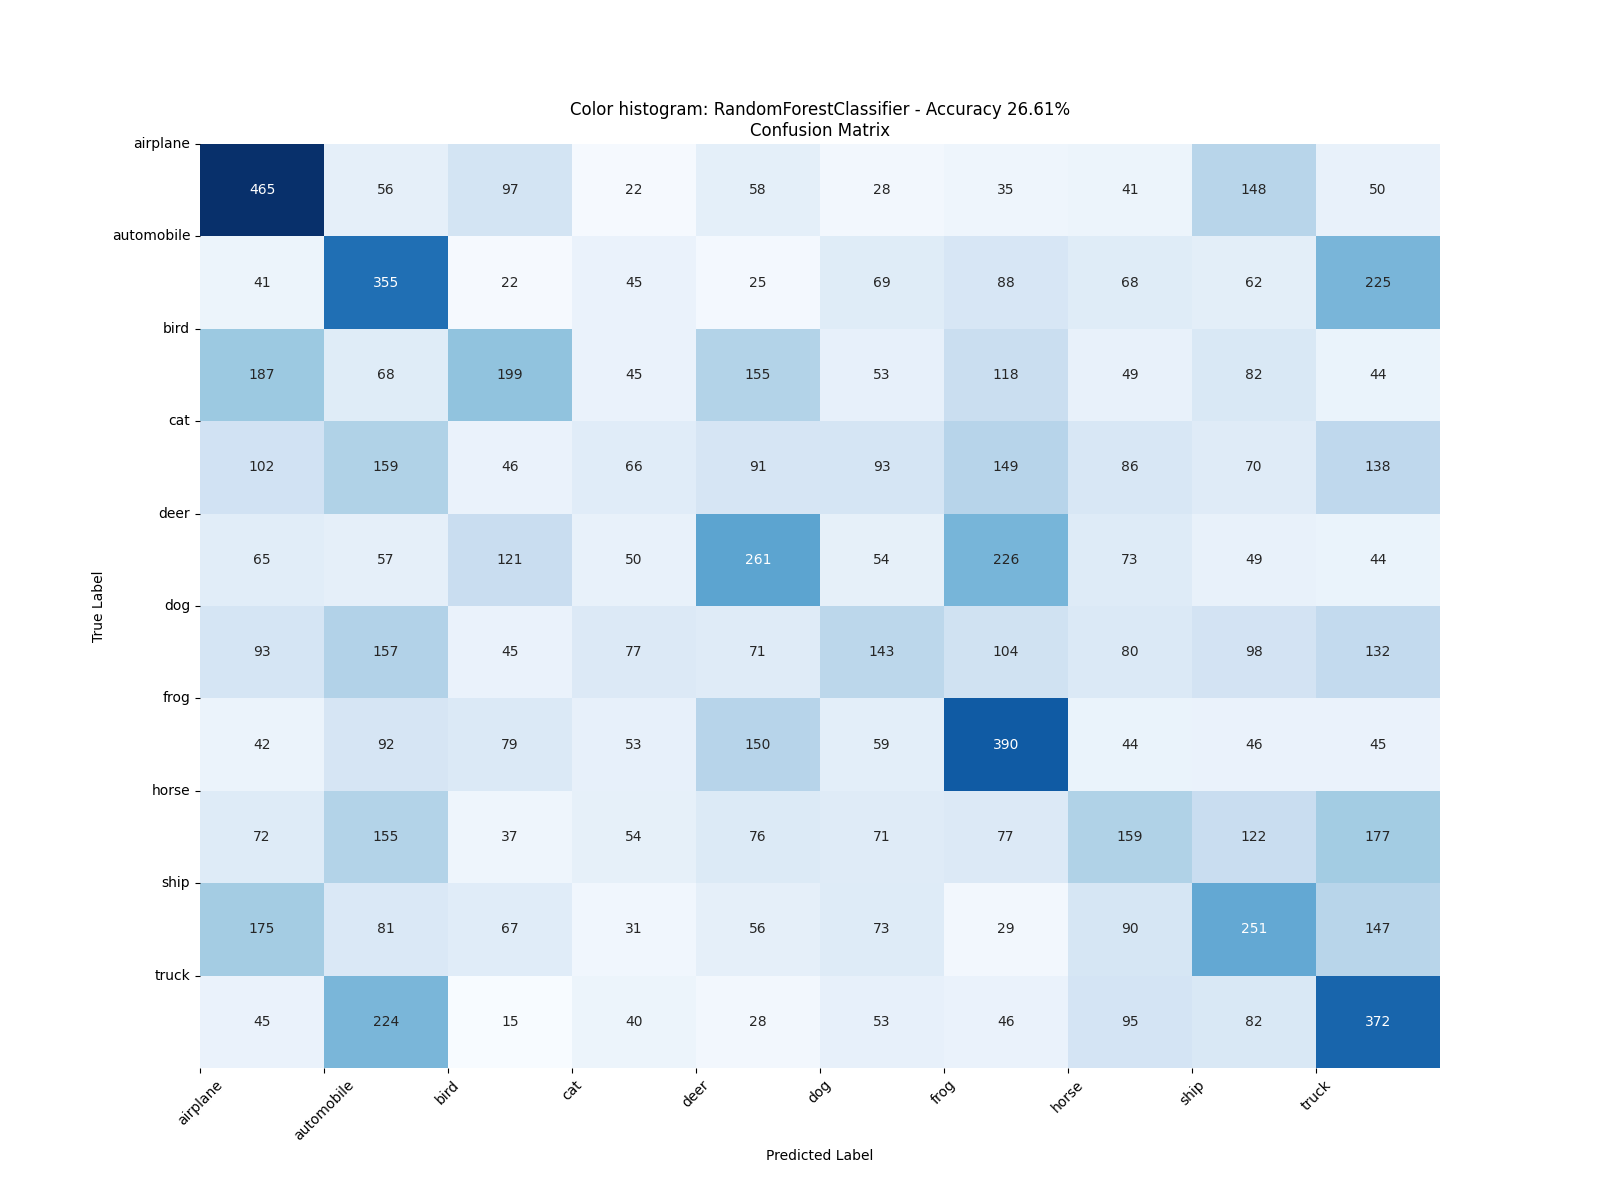
\includegraphics[scale=0.2]{figures/confusion_matrix_RandomForestClassifier_color.png}
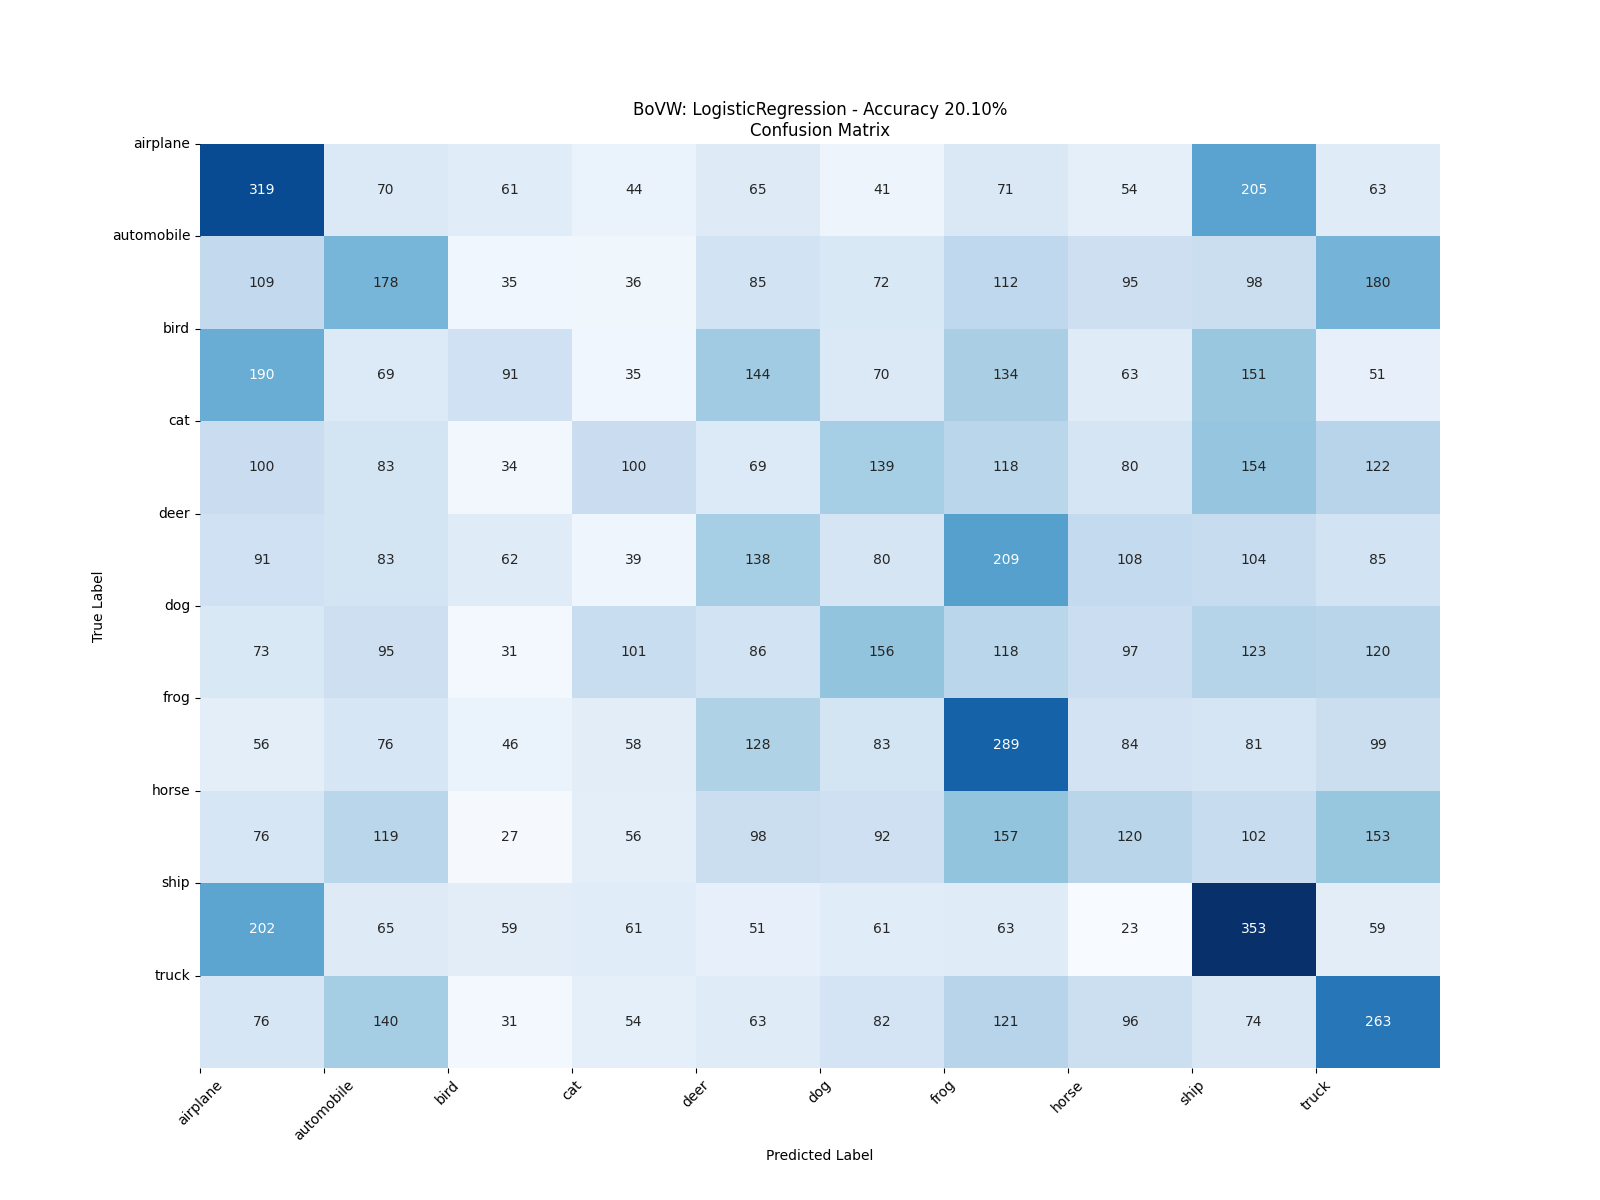
\includegraphics[scale=0.2]{figures/confusion_matrix_LogisticRegression_bovw_ft.png}
\caption{Matrice de confusion pour les meilleurs modèles selon la méthode d'extraction de features: Random forest sur image applatie (haut gauche), random forest sur histogramme de couleur (haut droite) et regression logistique sur \textit{BoVW} (bas)}
\label{fig:confusion}
\end{figure}

Maintenant, nous allons affiner les hyperparamètres pour le random forest sur l'image aplatie et l'histogramme de couleur et la régression logistique sur le \textit{BoVW} pour voir si cela peut améliorer les résultats de la classification. La Figure \ref{tab:fine_tuning} présente l'évolution de l'accuracy avec et sans affinage des hyperparamètres.

\begin{table}[ht]
\centering
\begin{tabular}{|c|c|c|c|}
\toprule
& RandomForest + Flatten & RandomForest + ColorHist & LogisticRegression + BoVW \\
\midrule
Sans fine-tuning & 47.01\% & 26.61\% & 20.41\% \\
Avec fine-tuning & 48.53\% & 27.98\% & 20.41\% \\
\bottomrule
\end{tabular}
\caption{Evolution de l'accuracy après affinage des hyperparamètres pour une régression logistique avec BoVW, et deux random forest avec image aplatie et histogramme de couleur.}
\label{tab:fine_tuning}
\end{table}
La régression logistique avec \textit{BoVW} ne progresse pas en affinant ses hyperapamètres, il semblerait que les paramètres par défauts produisent déjà les meilleurs résultats.
Pour les modèles sur utilisant les random forest, les résultats s'améliorent de manière intéressante, on atteint $48.53\%$ d'accuracy avec l'image aplatie.

Bien que les résultats présentés ici soient intéressants, nous n'avons pas utilisé d'apprentissage profond. Si on souhaite se comparer à l'état de l'art, \cite{kabir2023reduction} présente $99.70\%$ d'accuracy sur ce dataset utilisant les transformers. Nos résultats sont ridicules si on les compare simplement comme ça, mais il ne faut pas oublier que la méthode qui obtient le meilleur résultat ici est celle qui ne requiert strictement aucun pré-traitement des images, qui est donc légère. En limitant le nombre d'arbres dans le random forest, le modèle aussi peut être relativement léger, plus qu'un transformer en tout cas.
\section{Conclusion}

Dans ce rapport, nous avons comparé trois manières différentes d'extraire des informations d'une image, pour ensuite les utiliser dans trois différents modèles de classification. En entrainant et en comparant les modèles, nous avons remarqué qu'un pré-traitement trop lourd ne garantissait pas de meilleurs résultats sur le dataset CIFAR-10, et avait même l'effet inverse. Après affinage des hyperparamètres, nous avons atteint $48.53\%$ d'accuracy sur le jeu de test. Ces résultats peuvent être intéressants suivant les besoins et les objectifs que l'on cherche à atteindre. Ici, nos modèles et le pré-traitement d'images sont très légers comparés à des modèles d'apprentissage profond.

\bibliographystyle{splncs04}
\bibliography{bibl}

% Uncomment to change the background colors for the annexes
%\definecolor{mycolor}{rgb}{0.63, 0.94, 0.83}
%\pagecolor{mycolor}

\end{document}